%convert -coalesce launch.gif launch_%d.png
\documentclass{beamer}

\newcommand{\VEV}[1]{\langle#1\rangle}
\newcommand{\sst}{\left(1-\frac{2M}{r}\right)}
\newcommand{\sh}{\mathrm{shell}}
\newcommand{\be}{\begin{equation}}
\newcommand{\ee}{\end{equation}}
\newcommand{\bue}{\begin{equation}}
\newcommand{\eue}{\end{equation}}
\newcommand{\bc}{\begin{center}}
\newcommand{\ec}{\end{center}}
\newcommand{\bea}[1]{\begin{eqnarray}\label{#1}}
\newcommand{\eea}{\end{eqnarray}}
\newcommand{\bua}{\begin{eqnarray*}}
\newcommand{\eua}{\end{eqnarray*}}
\newcommand{\dd}[2]{{{d#1}\over{d#2}}}
\newcommand{\ddt}[1]{\dd{#1}{t}}
\newcommand{\dddt}[1]{\dd{^2#1}{t^2}}
\newcommand{\aver}[1]{\langle{#1}\rangle}
\newcommand{\atom}[3]{\ifmmode^{#1}_{#2}{\rm{#3}}\else{$^{#1}_{#2}${#3}}\fi}
\newcommand{\electron}{\atom{~0}{-1}{e}}
\newcommand{\positron}{\atom{0}{0}{\bar{e}}}
\newcommand{\neutrino}{\atom{0}{0}{\nu_e}}
\newcommand{\photon}{\atom{0}{0}{\gamma}}
\newcommand{\antineutrino}{\atom{0}{0}{\bar{\nu}}}
\newcommand{\neutron}{\atom{1}{0}{n}}
\newcommand{\proton}{\atom{1}{1}{p}}
\newcommand{\hydrogen}{\atom{1}{1}{H}}
\newcommand{\deuterium}{\atom{2}{1}{H}}
\newcommand{\tritium}{\atom{3}{1}{H}}
\newcommand{\helium}{\atom{4}{2}{He}}
\newcommand{\hethree}{\atom{3}{2}{He}}

\renewcommand{\ss}{Schwarz\-schild }

\def\densu{kg/m$^3$} 
\def\rsol{R$_{\odot}$} 
\def\msol{M$_{\odot}$} 


\usetheme{Boadilla}
%\usepackage{multimedia}
%\usepackage{animate}
\usepackage{hyperref}
\usepackage{tikz}
\usepackage{cancel}
\usepackage{tikzsymbols}
\usepackage{ifthen}

%%%%mathcircled
\makeatletter
\newcommand\mathcircled[1]{%`
  \mathpalette\@mathcircled{#1}%
}
\newcommand\@mathcircled[2]{%
  \tikz[baseline=(math.base)] \node[draw,circle,red, thick, inner sep=2pt] (math) {$\m@th#1#2$};%
}
\makeatother
%%%%

%gets rid of bottom navigation bars
\setbeamertemplate{footline}[frame number]{} %begin

%gets rid of bottom navigation symbols
\setbeamertemplate{navigation symbols}{}

%gets rid of footer
%will override 'frame number' instruction above  %begin
%comment out to revert to previous/default definitions
\setbeamertemplate{footline}{}

\definecolor{darkscarlet}{rgb}{0.34, 0.01, 0.1}
\definecolor{gold(metallic)}{rgb}{0.83, 0.69, 0.22}
\definecolor{green(ryb)}{rgb}{0.4, 0.69, 0.2}
\definecolor{darkorange}{rgb}{1.0, 0.55, 0.0}
\definecolor{amber}{rgb}{1.0, 0.75, 0.0}
\definecolor{bronze}{rgb}{0.8, 0.5, 0.2}
\definecolor{cadet}{rgb}{0.33, 0.41, 0.47}
\definecolor{silver}{rgb}{0.75, 0.75, 0.75}
\definecolor{turquoise}{rgb}{0.19, 0.84, 0.78}
\definecolor{uclagold}{rgb}{1.0, 0.7, 0.0}
\definecolor{urobilin}{rgb}{0.88, 0.68, 0.13}
\definecolor{vegasgold}{rgb}{0.77, 0.7, 0.35}
\definecolor{vanilla}{rgb}{0.95, 0.9, 0.67}
\definecolor{straw}{rgb}{0.89, 0.85, 0.44}
\definecolor{sunset}{rgb}{0.98, 0.84, 0.65}
\definecolor{brown(traditional)}{rgb}{0.59, 0.29, 0.0}
\definecolor{apricot}{rgb}{0.98, 0.81, 0.69}
\definecolor{darkblue}{rgb}{0,0,0.54}

\hypersetup{
    colorlinks=true,
    linkcolor=yellow,
    filecolor=magenta,
    urlcolor=blue,
}

\let\hrefori\href
\renewcommand{\href}[2]{{\setlength{\fboxsep}{1pt}\colorbox{sunset}{\hrefori{#1}{#2}}}}


%title
\setbeamercolor{block title alerted}{fg=white,bg=cyan}
%body
\setbeamercolor{block body alerted}{fg=black!90,bg=yellow!60}

%title
\setbeamercolor{block title}{fg=black,bg=turquoise}
%body
\setbeamercolor{block body}{fg=yellow,bg=bronze}




\newcommand{\pagebutton}[1]{\setbeamertemplate{button}{\tikz\node[inner xsep = 5pt, draw = structure!90, fill = green(ryb), rounded corners = 8pt]{\color{amber}\Large\insertbuttontext};}\beamerbutton{#1}}

\newcommand{\choicebutton}[1]{\setbeamertemplate{button}{\tikz\node[inner xsep = 8pt, draw = structure!90, fill = vegasgold, rounded corners = 5pt]{\color{vanilla}\Large\insertbuttontext};}\beamerbutton{#1}}

\newcommand{\pagenobutton}[1]{\setbeamertemplate{button}{\tikz\node[inner xsep = 8pt, draw = structure!90, fill = apricot, rounded corners = 5pt]{\color{brown(traditional)}\Large\insertbuttontext};}\beamerbutton{#1}}

\newcommand{\headlinebutton}[1]{\setbeamertemplate{button}{\tikz\node[inner xsep = 8pt, draw = structure!90, fill = blue, rounded corners = 5pt]{\color{yellow}\Large\insertbuttontext};}\beamerbutton{#1}}

\newcommand{\forumbutton}{\href{https://astro-discourse.utenforuio.no/c/ast2000/sporsmal-til-ukeoppgavene-i-del-2a-2d/11}{\setbeamertemplate{button}{\tikz\node[inner xsep = 8pt, draw = structure!90, fill = darkblue, rounded corners = 5pt]{\color{yellow}\Large\insertbuttontext};}\beamerbutton{\textcolor{red}{\small FORUM}}}}

\newcommand{\curpage}{\pagenobutton{\small side \thepageno\  av \thenopages}}
\newcommand{\nextpage}{\refstepcounter{pageno}\pagenobutton{\small side \thepageno\  av \thenopages}}
\newcommand{\dnextpage}{\refstepcounter{pageno}\refstepcounter{pageno}\pagenobutton{\small side \thepageno\  av \thenopages}}

\newcommand{\lastpagebutton}[1]{\hyperlink{#1}{\pagebutton{\small Forrige side}}\href{https://nettskjema.no/a/171403}{\Changey[1][yellow]{2} \Changey[1][yellow]{-2}}\nextpage\headlinebutton{\headline}\forumbutton}
\newcommand{\clastpagebutton}[1]{\hyperlink{#1}{\pagebutton{\small Forrige side}}\href{https://nettskjema.no/a/171403}{\Changey[1][yellow]{2} \Changey[1][yellow]{-2}}\curpage\headlinebutton{\headline}\forumbutton}
\newcommand{\dlastpagebutton}[1]{\hyperlink{#1}{\pagebutton{\small Forrige side}}\href{https://nettskjema.no/a/171403}{\Changey[1][yellow]{2} \Changey[1][yellow]{-2}}\dnextpage\headlinebutton{\headline}\forumbutton}

\newcommand{\lastpagebuttonx}[1]{\hyperlink{#1}{\pagebutton{\small Forrige side}}\href{https://nettskjema.no/a/171403}{\Changey[1][yellow]{2} \Changey[1][yellow]{-2}}\nextpage\\}
\newcommand{\clastpagebuttonx}[1]{\hyperlink{#1}{\pagebutton{\small Forrige side}}\href{https://nettskjema.no/a/171403}{\Changey[1][yellow]{2} \Changey[1][yellow]{-2}}\curpage\\}
\newcommand{\dlastpagebuttonx}[1]{\hyperlink{#1}{\pagebutton{\small Forrige side}}\href{https://nettskjema.no/a/171403}{\Changey[1][yellow]{2} \Changey[1][yellow]{-2}}\dnextpage\\}

\newcommand{\lastpagebuttoncr}[1]{\hyperlink{#1}{\pagebutton{\small Forrige side}}\href{https://nettskjema.no/a/171403}{\Changey[1][yellow]{2} \Changey[1][yellow]{-2}}\nextpage\\\headlinebutton{\headline}\forumbutton\\}
\newcommand{\clastpagebuttoncr}[1]{\hyperlink{#1}{\pagebutton{\small Forrige side}}\href{https://nettskjema.no/a/171403}{\Changey[1][yellow]{2} \Changey[1][yellow]{-2}}\curpage\\\headlinebutton{\headline}\forumbutton\\}
\newcommand{\dlastpagebuttoncr}[1]{\hyperlink{#1}{\pagebutton{\small Forrige side}}\href{https://nettskjema.no/a/171403}{\Changey[1][yellow]{2} \Changey[1][yellow]{-2}}\dnextpage\\\headlinebutton{\headline}\forumbutton\\}

\newcommand{\nytemaside}[1]{
\centerline{\Huge\textcolor{yellow}{Nytt tema:}}\\
\vspace*{1cm}
\centerline{\Large\bf\textcolor{yellow}{\headline}}
\vspace*{2cm}
\ifthenelse{\equal{#1}{0}}{\centerline{\textcolor{yellow}{Siste tema i denne forelesningen!}}}{\centerline{\textcolor{yellow}{\footnotesize Dette temaet fortsetter frem til side \ref{#1} av \thenopages.}}}
\vspace*{0.5cm}
}


\newcommand{\fullframe}[6]{
\begin{frame}
\label{#1}
\addtocounter{pageno}{#4}
\lastpagebutton{#2}{\bf #6}\\
#5
\hyperlink{#3}{\pagebutton{Neste side}}
\end{frame}
}



\newcommand{\fullframetwo}[7]{
\begin{frame}
\label{#1}
\addtocounter{pageno}{#4}
\lastpagebutton{#2}{\bf #7}\\
\begin{columns}
\column{0.5\textwidth}
#5
\column{0.5\textwidth}
#6
\hyperlink{#3}{\pagebutton{Neste side}}
\end{columns}
\end{frame}
}

\newcommand{\fullframetwonotxt}[7]{
\begin{frame}
\label{#1}
\addtocounter{pageno}{#4}
\lastpagebutton{#2}{\bf #7}\\
\begin{columns}
\column{0.5\textwidth}
#5
\column{0.5\textwidth}
#6
\end{columns}
\end{frame}
}



\newcommand{\fullframetxt}[7]{
\begin{frame}
\label{#1}
\addtocounter{pageno}{#4}
\lastpagebutton{#2}{\bf #7}\\
#6
\hyperlink{#3}{\pagebutton{#5}}
\end{frame}
}

\newcommand{\fullframenotxt}[6]{
\begin{frame}
\label{#1}
\addtocounter{pageno}{#4}
\lastpagebutton{#2}{\bf #6}\\
#5
\end{frame}
}

\newcommand{\choiceframe}[5]{
\begin{frame}
\label{#1}
\addtocounter{pageno}{#3}
\lastpagebutton{#2}{\bf #5}\\
#4
\end{frame}
}

\newcommand{\colfullframe}[7]{
{
\setbeamercolor{background canvas}{bg=#5}
\begin{frame}
\label{#1}
\addtocounter{pageno}{#4}
\lastpagebutton{#2}{\bf #7}\\
#6
\hyperlink{#3}{\pagebutton{Neste side}}
\end{frame}
}
}

\newcommand{\colfullframetwo}[8]{
{
\setbeamercolor{background canvas}{bg=#5}
\begin{frame}
\label{#1}
\addtocounter{pageno}{#4}
\lastpagebutton{#2}{\bf #8}\\
\begin{columns}
\column{0.5\textwidth}
#6
\column{0.5\textwidth}
#7
\hyperlink{#3}{\pagebutton{Neste side}}
\end{columns}
\end{frame}
}
}

\newcommand{\colfullframetxt}[8]{
{
\setbeamercolor{background canvas}{bg=#5}
\begin{frame}
\label{#1}
\addtocounter{pageno}{#4}
\lastpagebutton{#2}{\bf #8}\\
#7
\hyperlink{#3}{\pagebutton{#6}}
\end{frame}
}
}

\newcommand{\colchoiceframe}[6]{
{
\setbeamercolor{background canvas}{bg=#4}
\begin{frame}
\label{#1}
\addtocounter{pageno}{#3}
\lastpagebutton{#2}{\bf #6}\\
#5
\end{frame}
}
}


\newcommand{\pagequestion}[3]{
\hyperlink{#1}{\pagebutton{#2}}
\pause
%#3 normalt -1 for første spørsmål
\addtocounter{pageno}{#3}
\begin{itemize}[<+->]
\item[] \hypertarget<.>{#1}{}
\end{itemize}
\vspace{-0.5cm}
}

\newcommand{\samepagequestion}[4]{
\hyperlink{#1}{\pagebutton{#2}}\hyperlink{#1}{\pagebutton{#3}}
\pause
%#3 normalt -1 for første spørsmål
\addtocounter{pageno}{#4}
\begin{itemize}[<+->]
\item[] \hypertarget<.>{#1}{}
\end{itemize}
\vspace{-0.5cm}
}

\newcommand{\twopagequestion}[7]{
\hyperlink{#1}{\pagebutton{#3}}\hyperlink{#2}{\pagebutton{#4}}
\pause
%#3 normalt -1 for første spørsmål
\addtocounter{pageno}{#5}
\begin{itemize}[<+->]
\item[] \hypertarget<.>{#1}{}
\end{itemize}
\vspace{-0.5cm}
#7
\addtocounter{pageno}{#6}
\begin{itemize}[<+->]
\item[] \hypertarget<.>{#1}{}
\end{itemize}
\vspace{-0.5cm}
}

\newcounter{pageno}
\newcounter{nopages}
\setcounter{nopages}{42}

\newcommand{\headline}{\small Introduksjon}
\newcommand{\m}{\mathrm{m}}

\begin{document}

\begin{frame}
\label{front2}
\center{\Large \textcolor{darkscarlet}{\bf AST2000 Del 2B\\Interaktive forelesningsnotater: forelesning 1 av 2}}\\
\begin{block}{\center{\bf VIKTIG}}
\textcolor{yellow}{Dette er et alternativ til forelesningen i emnet.} \textcolor{blue}{Har du gått skikkelig gjennom disse interaktive forelesningsnotatene så trenger du ikke å lese \href{https://www.uio.no/studier/emner/matnat/astro/AST2000/h21/undervisningsmateriell/lecture_notes/part2b.pdf}{de fulle forelesningsnotatene} (med unntak av oppgavene bak)}. All informasjonen du trenger, får du her. Du kommer til å få mange grublespørsmål og diskusjonsoppgaver, det er meningen at disse skal gjøres i grupper av minst 2, maks 4 studenter. {\bf Det er defor sterkt anbefalt at dere sitter sammen i grupper når dere går gjennom disse interaktive forelesningsnotatene, du vil få betydelig mer utbytte av dem på den måten}. {\bf Hvis du har kommentarer ris/ros til disse forelesningsnotatene eller til emnet, trykk på \href{https://nettskjema.no/a/171403}{\Changey[1][yellow]{2} \Changey[1][yellow]{-2}}\ knappen som du finner på alle sider.}
\end{block}
%\setbeamercolor{button}{bg=black,fg=yellow}
\hyperlink{front3}{\pagebutton{Trykk denne knappen for å begynne}}
\end{frame}

\begin{frame}
\label{front3}
{\Large
\begin{itemize}
\item HUSK at du får mer ut av de interaktive forelesningsnotatene når du gjør de sammen med noen. Diskusjonene med andre er svært viktige.
\item Det er mange spørsmål/grubliser underveis, sett dere selv en tidsgrense, 1 minutt på de korte, maks 4-5 minutter på de lenger. Ha en alarm ved siden av, ellers kommer dere til å bruke alt for langt tid. Har dere ikke fått det til etter kort tid, gå videre, se svaret og lær!
\item Er du i det minste tvil om noe, så finnes det en \forumbutton knapp, trykk det og still spørsmål med en gang mens du enda husker spørsmålet!
\end{itemize}
}
\hyperlink{tableofcontents}{\pagebutton{Trykk denne knappen for å begynne}}
\end{frame}

\begin{frame}
\label{tableofcontents}
\hyperlink{front3}{\pagebutton{Forrige side}}\\
Hvis du allerede har begynt på denne forelesningen og vil hoppe rett inn til et annet kapittel, kan du trykke her:
\begin{itemize}
\item \hyperlink{blue_nytema1}{\headlinebutton{}}
\item \hyperlink{blue_nytema2}{\headlinebutton{}}
\item \hyperlink{blue_nytema3}{\headlinebutton{}}
\end{itemize}
Merk at sidene er merket med sidenummer på denne måten: SIDE X/Y/Z. Her er Z antall sider totalt, Y er sidenummeret til siste side i avsnittet du holder på med og X er sidenummeret til siden du er på.\\
\hyperlink{intro}{\choicebutton{Neste side}}
\end{frame}


%%%%% intro
\begin{frame}
\label{intro}
\begin{columns}
\column{0.5\textwidth}
\hyperlink{front}{\pagebutton{Forrige side}}\\

\includegraphics[scale=0.25]{media/clock.png}
\column{0.5\textwidth}
{\small
{\bf Velkommen til forelesning 1 av 2 i del 2B! I denne første forelesningen skal vi se nærmere på fremstilling av eventer i tid og rom og avstander mellom slike i et tidromdiagram. Vi skal forsøke å forstå litt mer av hva tidromsavstanden $\Delta s$ sier oss. Til slutt skal vi introdusere 4-vektorer som er 4-dimensjonale vektorer i tidrommet.}\\
\textcolor{red}{Fremstillingen av spesiell relativitetsteori i AST2000 er basert på den fantastiske boken ``Spacetime Physics'' av E. Taylor og J. Wheeler, gratis tilgjengelig \href{http://www.eftaylor.com/spacetimephysics/}{her}. Anbefales på det sterkeste for den som er interessert.}
{(\tiny Illustrasjon fra pngegg.com)}}
\hyperlink{intro2}{\pagebutton{Neste side}}
\end{columns}
\end{frame}



\begin{frame}`
\label{intro2}
\lastpagebutton{intro}
\begin{alertblock}{Vi begynner som vanlig...}
...med litt brainstorming. Som det er {\bf svært viktig} at du gjør før du går videre.
\end{alertblock}
\href{https://nettskjema.no/a/171333}{\begin{minipage}{5cm}Trykk her for å varme opp\end{minipage}}\\
Er du klar og har sendt inn skjemaet?
\href{https://nettskjema.no/a/171333}{\choicebutton{Nei}}\ \ \ \ \hyperlink{brainstormdone}{\choicebutton{Ja}}\\
%\hyperlink{intro2}{\choicebutton{Nei}}\ \ \ \ \hyperlink{brainstormdone}{\choicebutton{Ja}}\\
\pause
\addtocounter{pageno}{-1}
\begin{itemize}[<+->]
\item[] \hyperlink{blue_nytema1}{\pagebutton{Neste side}} \hypertarget<.>{brainstormdone}{}
\end{itemize}
\end{frame}





\renewcommand{\headline}{Tidromdiagram}
{
\setbeamercolor{background canvas}{bg=blue}
\begin{frame}
\label{blue_nytema1}
\hyperlink{intro2}{\pagebutton{\small Forrige side}}
\nytemaside{maksaldring}
\textcolor{yellow}{\Large Og vi skal ta en pause før vi kommer helt frem til neste tema!}
\hyperlink{td1}{\pagebutton{La oss starte reisen i tid og rom...}}
\end{frame}
}


\fullframe{td1}{intro2}{td2}{1}{\Huge

Vi skal begynne med å lære om {\bf verdenslinjer}. Se \href{https://www.uio.no/studier/emner/matnat/astro/AST2000/h20/undervisningsmateriell/interaktive-forelesningsnotater/2b/videoer/video2b_1.mp4}{denne videoen} for å se hva verdenslinjer er for noe...
}

\fullframetxt{td2}{td1}{td3}{0}{Du må ha et forslag før du går videre}{\small
\centerline{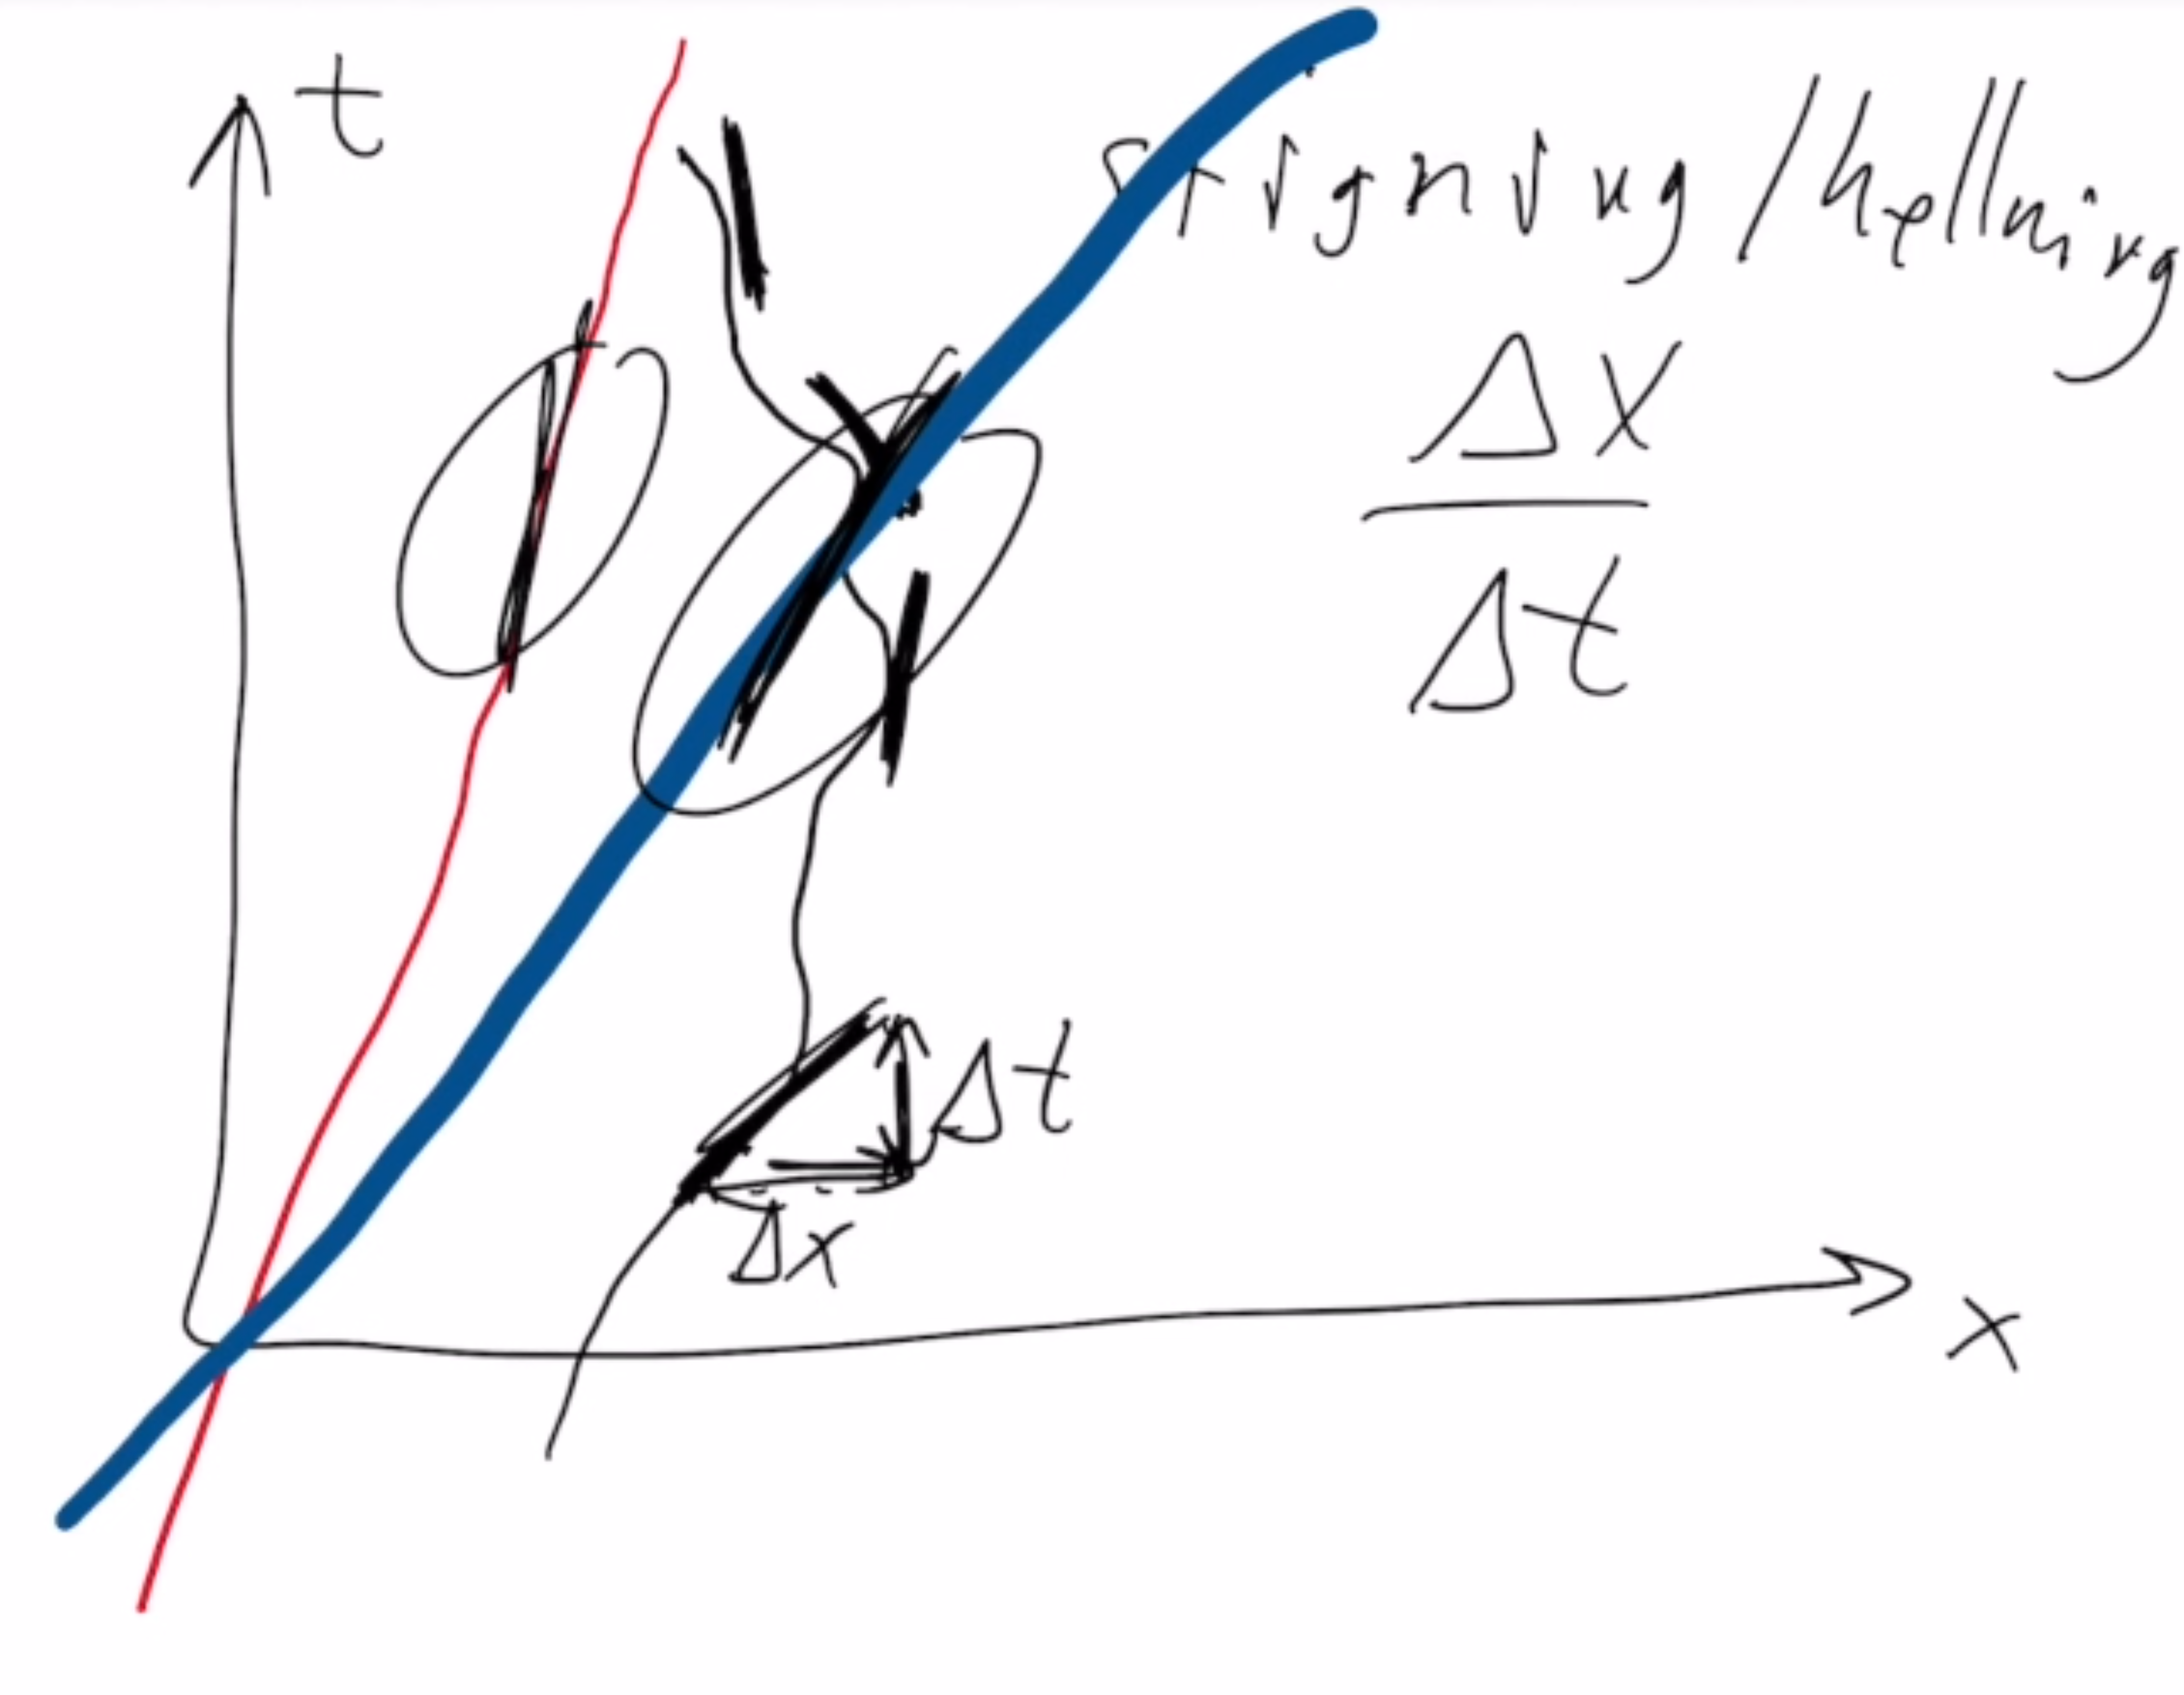
\includegraphics[scale=0.17]{media/hellning.png}}
Vi sluttet videoen med denne figuren. Og med spørsmålet om hva helningen/stigningen til verdenslinjene betyr fysisk. Merk at vi definerer stigningen her som økning langs x-akse delt på endring langs y-akse. Vi ser her to rette linjer, rød og blå, som er verdenslinjene til to forskjellige observatører. Hva er forskjellig for disse observatørene? Hva betyr det at helningen til linjene deres er forskjellig? Tenk deg godt om før du går videre!
}


\choiceframe{td3}{td2}{0}{
Er du med på at {\bf farta} til objektet som verdenslinja representerer er avgjørende for helninga? Endring langs x-aksen, altså $\Delta x$, delt på endring langs t-aksen $\Delta t$ blir vel $v$?
\[
v=\frac{\Delta x}{\Delta t}
\]
Det kan men vel se for seg: hvis verdenslinja går rett opp, så er det ingen endring i $x$ med tiden, da må vi ha $v=0$. Og hvis verdenslinja svinger litt slik at $x$-posisjon endres, så må det være en hastighet. Hvilken helning har da verdenslinja til lys?\\
\hyperlink{feil_td3a}{\choicebutton{det er en horisontal linje}}
\hyperlink{feil_td3a}{\choicebutton{det er en vertikal linje}}
\hyperlink{feil_td3a}{\choicebutton{linja danner 22.5 grader med x-aksen}}
\hyperlink{feil_td3a}{\choicebutton{linja danner 30 grader med x-aksen}}
\hyperlink{riktig_td3b}{\choicebutton{linja danner 45 grader med x-aksen}}
\hyperlink{feil_td3a}{\choicebutton{linja danner 67.5 grader med x-aksen}}
}


\colchoiceframe{feil_td3a}{td3}{0}{black}{\Huge
\textcolor{yellow}{Hmmmmmm...tenk igjen! Husk hvordan man omgjør et tidsintervall målt i sekunder til meter! Hvis du nå har meter for avstander i både tid og rom, hvor langt $\Delta x$ beveger lys seg i løpet av en tid $\Delta t$? Si at $\Delta x$ er 1 meter?}
}

\colfullframe{riktig_td3b}{td3}{td4}{-1}{yellow}{\large
Det er helt riktig! Når vi bruker samme enheter i både tid og rom så er jo $v$ et tall mellom 0 og 1 (gå tilbake til forrige forelesning hvis du ikke husker hvorfor, dette er {\bf svært} viktig å ha kontroll over for å kunne forstå resten av denne forelesningen! Vi fant der at lyshastigheten tilsvarer $v=1$. Hvis $v=1$ så må dermed $\Delta x = \Delta t$ (utifra definisjonen av $v$ på forrige side). Det betyr at lys alltid beveger seg like langt i rom som i tid. Og da får vi en helning på 45 grader.
}


\fullframe{td4}{riktig_td3b}{td5}{0}{\Huge
\centerline{
\includegraphics[scale=0.6]{media/cowboy.png}}
Så til en litt voldlig episode i \href{https://www.uio.no/studier/emner/matnat/astro/AST2000/h20/undervisningsmateriell/interaktive-forelesningsnotater/2b/videoer/video2b_2.mp4}{denne videoen}...
}

\choiceframe{td5}{td4}{0}{\Huge
%\centerline{\includegraphics[scale=0.3]{media/}}
Så i hvilke(t) event kan det være at personen faller om som følge av skuddet? Du har lov til å sette betingelser på våpnet her, innenfor hva som er tillatt i fysikk.\\
\hyperlink{feil_td5a}{\choicebutton{Bare B}}
\hyperlink{feil_td5a}{\choicebutton{Bare C}}
\hyperlink{feil_td5a}{\choicebutton{Bare D}}
\hyperlink{riktig_td5b}{\choicebutton{B og C}}
\hyperlink{feil_td5a}{\choicebutton{B og D}}
\hyperlink{feil_td5a}{\choicebutton{C og D}}
\hyperlink{feil_td5a}{\choicebutton{alle tre}}
}

\colchoiceframe{feil_td5a}{td5}{0}{black}{\huge
\textcolor{yellow}{Det ble nok galt! Prøv å trekke en linje fra event A til hver av de andre eventene. Hva slags helning er det på linja? Kan et prosjektil følge en slik verdenslinje? (lasterpistol er jo også en mulighet...) Hvis du kommer hit for andre gang, se på \href{https://www.uio.no/studier/emner/matnat/astro/AST2000/h20/undervisningsmateriell/interaktive-forelesningsnotater/2b/videoer/video2b_3.mp4}{denne videoen}}
}

\colfullframe{riktig_td5b}{td5}{td6}{-1}{yellow}{\Huge
Det var riktig. Er du likevel i tvil kan du se på \href{https://www.uio.no/studier/emner/matnat/astro/AST2000/h20/undervisningsmateriell/interaktive-forelesningsnotater/2b/videoer/video2b_3.mp4}{denne videoen}
}



\fullframe{td6}{riktig_td5b}{td7}{0}{\Large
Event A og de tre andre eventene er ekesmpler på det vi kaller {\bf tidlike}, {\bf lyslike} og {\bf romlike} eventer. Vi skal nå se på betydningen av hver av disse, en av gangen...
}

\fullframe{td7}{td6}{td8}{0}{
\begin{block}{Tidlike eventer...}
... er eventer som kan være {\bf kausalt forbundet}, dvs. at det ene eventet kan ha forårsaket det andre. For at det skal være mulig så må et objekt (f.eks. et prosjektil) kunne ha beveget seg fra det ene eventet til det andre i tide for at det andre eventet skal kunne skje. Dvs. at man må kunne trekke en rett linje, som i teorien tilsvarer verdenslinjen til et objekt, fra det ene eventet til det andre som har en helning slik at hastigheten $v<1$. Event A og B i eksemplet var dermed slike {\bf tidlike eventer}.
\end{block}
Hvis linjen vi trekker fra det ene eventet til den andre er en rett linje som i teorien tilsvarer $v<1$ så betyr det at x-avstanden $\Delta x$ mellom eventene må være mindre enn tidsavstanden $\Delta t$ (forstår du dette? Se på helningen til linja!) Dermed får vi et tidromsintervall
\[
\Delta s^2 = \Delta t^2 - \Delta x^2>0
\]
som er reelt, altså at $\Delta s^2>0$ er positivt og større enn null.
}



\fullframe{td8}{td7}{td9}{0}{
\begin{block}{Lyslike eventer...}
... er eventer som kan være {\bf kausalt forbundet}, dvs. at det ene eventet kan ha forårsaket det andre, men kun noe som beveger seg med lysets hastighet kan ha beveget seg fra det ene eventet og forårsaket det andre. Dvs. at man må kunne trekke en rett linje, som i teorien tilsvarer verdenslinjen til et objekt, fra det ene eventet til det andre som har en helning som tilsvarer lyshastigheten $v=1$, altså en linje som danner $45^\circ$ med x-aksen. Event A og C i eksemplet var dermed slike {\bf lyslike eventer}.
\end{block}
Hvis linjen vi trekker fra det ene eventet til den andre er en rett linje som i teorien tilsvarer $v=1$ så betyr det at x-avstanden $\Delta x$ mellom eventene må være lik tidsavstanden $\Delta t$. Dermed får vi et tidromsintervall
\[
\Delta s^2 = \Delta t^2 - \Delta x^2=0.
\]
Lys beveger seg slik at avstanden det tilbakelegger i det 4-dimensjonale tidrommet er 0.
}

\fullframe{td9}{td8}{td10}{0}{
\begin{block}{Romlike eventer...}
... er eventer som {\bf ikke} kan være {\bf kausalt forbundet}, dvs. at det ene eventet {\bf ikke} kan ha forårsaket det andre. Hvis man dermed trekker en rett linje, som i teorien tilsvarer verdenslinjen til et objekt, fra det ene eventet til det andre, så vil denne verdenslinja tilsvare en hastighet som er større en lysets $v>1$. Altså en helning med x-aksen som er mindre enn $45^\circ$. Ingen objekter kan bevege seg fortere enn lyset og dermed finnes det heller ingen objekter som kan følge denne verdenslinja og kausalt forbinde disse to eventene. Event A og D i eksemplet var dermed slike {\bf romlike eventer}.
\end{block}
Hvis linjen vi trekker fra det ene eventet til den andre er en rett linje som i teorien tilsvarer $v>1$ så betyr det at x-avstanden $\Delta x$ mellom eventene er {\bf større} enn tidsavstanden $\Delta t$. Dermed får vi et tidromsintervall
\[
\Delta s^2 = \Delta t^2 - \Delta x^2<0.
\]
Tidromsavstanden blir i dette tilfellet et imaginært tall. Det betyr at to romlike eventer ikke kan ligge på en og samme verdenslinje.
}


\fullframe{td10}{td9}{td11}{0}{\Large\bf
\textcolor{red}{Nå skal du få en ny problemstilling her i \href{https://www.uio.no/studier/emner/matnat/astro/AST2000/h20/undervisningsmateriell/interaktive-forelesningsnotater/2b/videoer/video2b_4.mp4}{denne videoen}.} Videoen avslutter slik:
\centerline{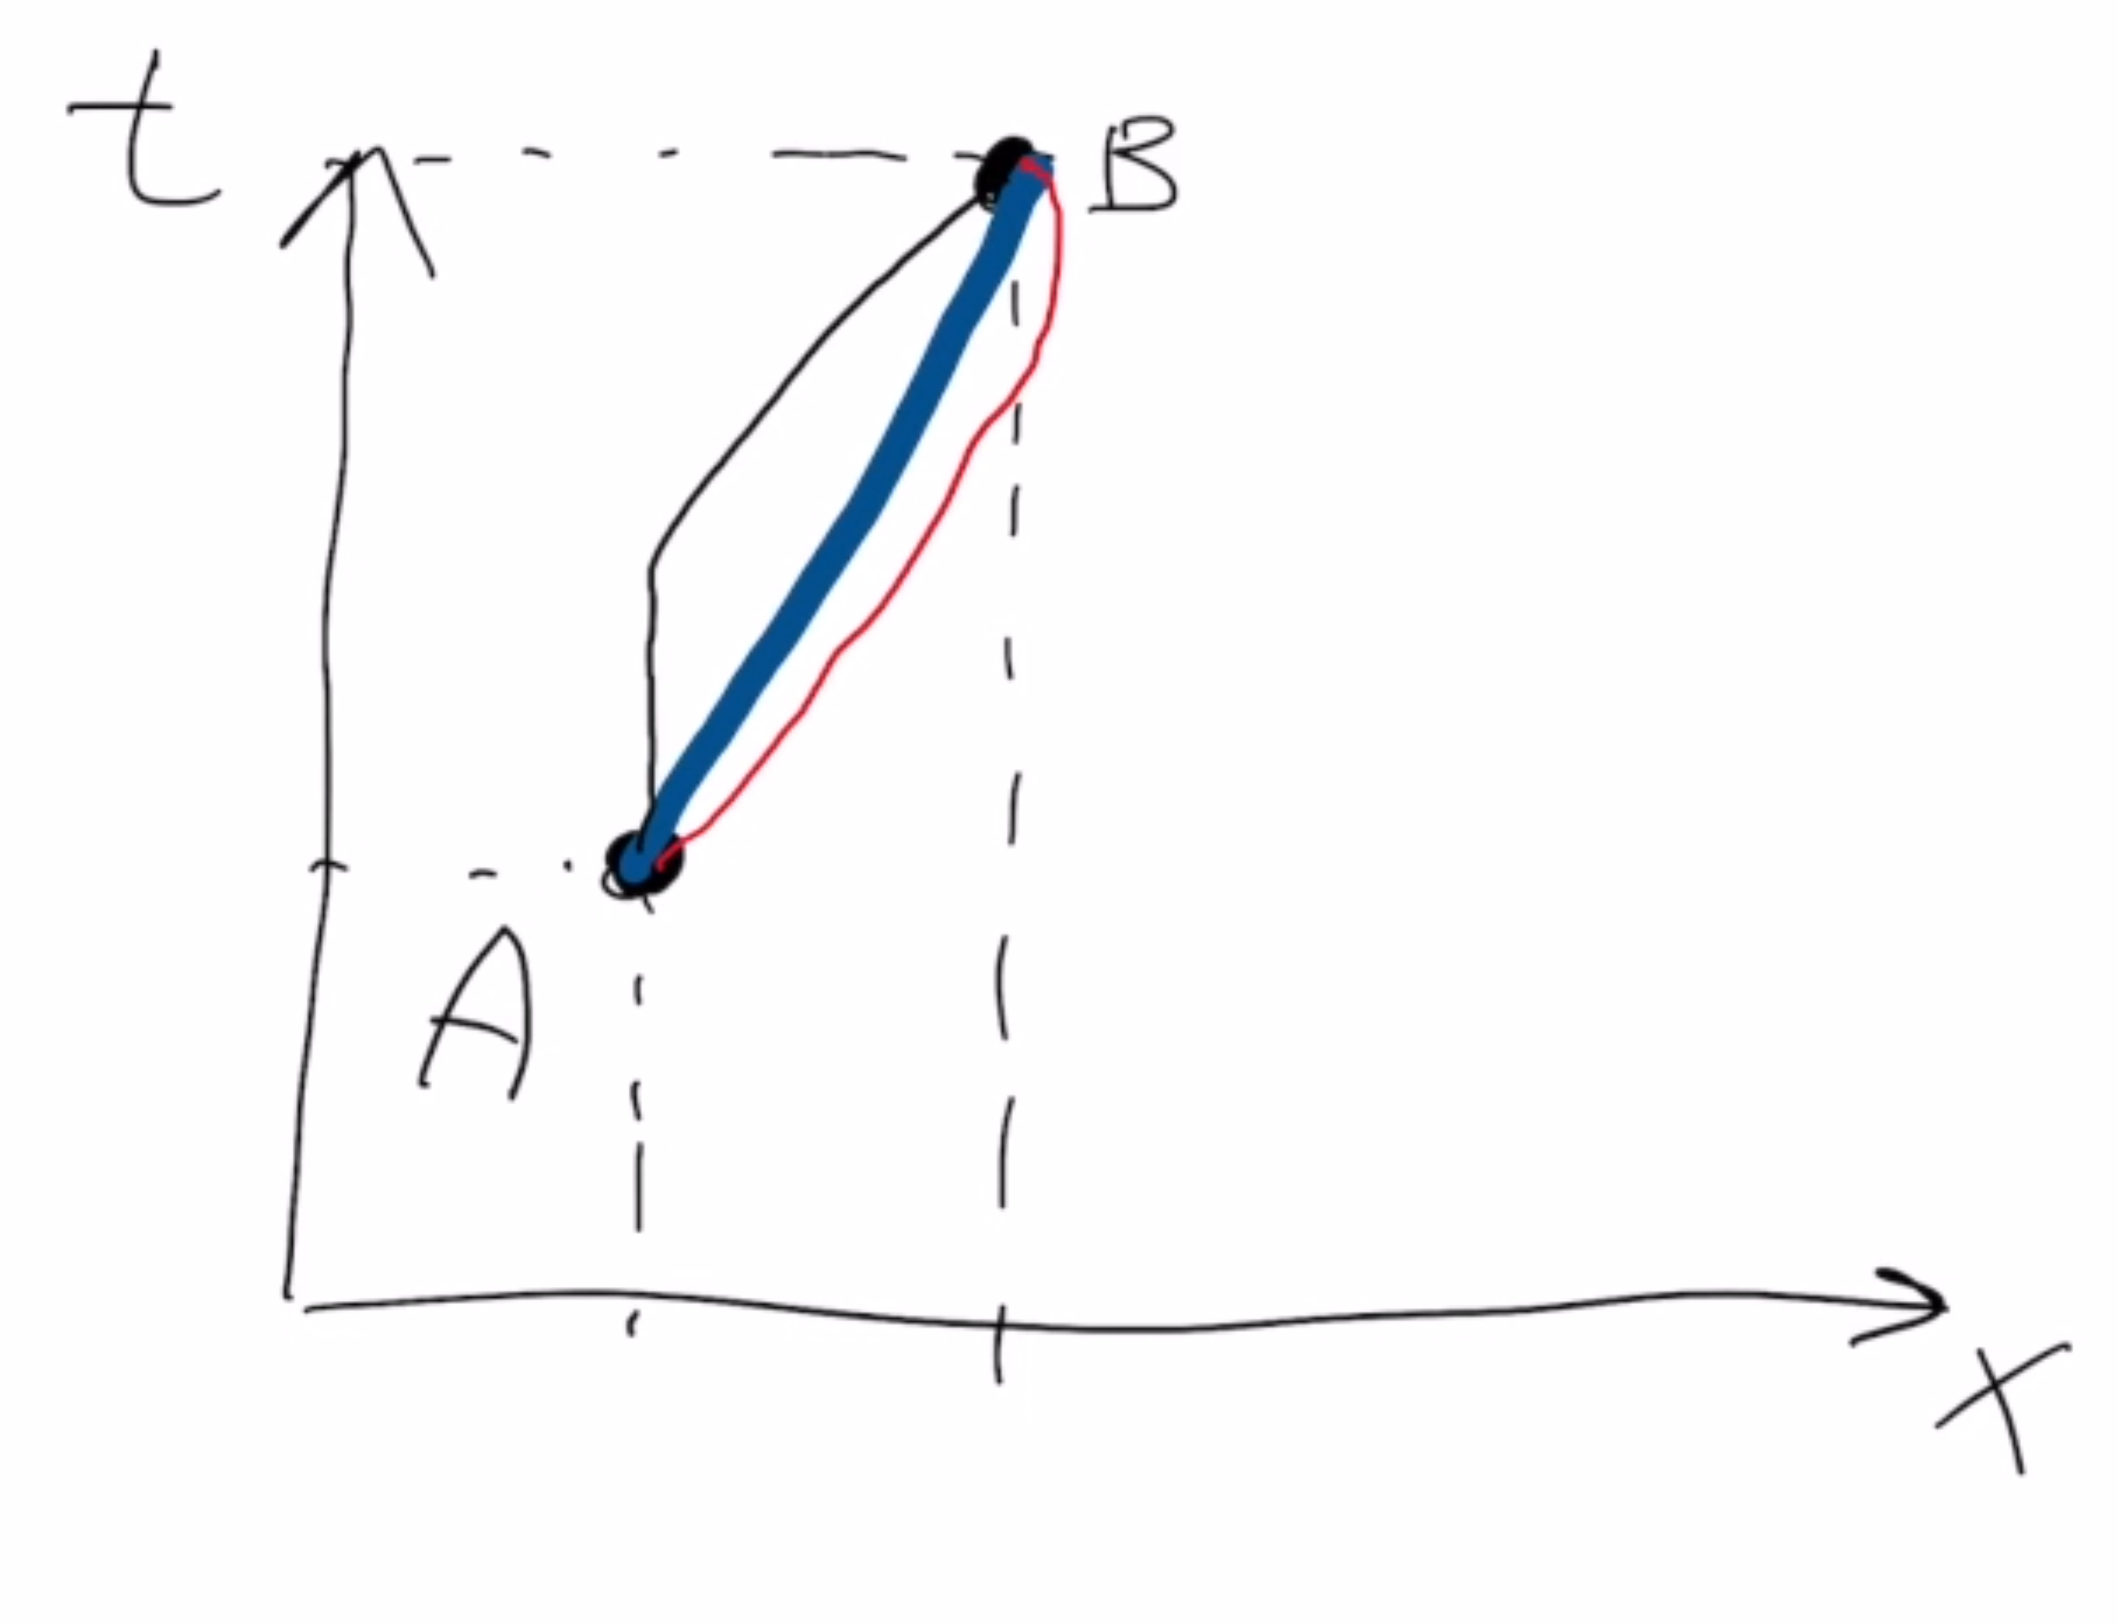
\includegraphics[scale=0.22]{media/cars.png}}
}


\choiceframe{td11}{td10}{0}{
%\centerline{\includegraphics[scale=0.3]{media/}}
Hva ble riktig her? Med ``akselererer mest så menes ``har aller størst akselrasjon i løpet av et kort tidsrom, dvs. har den største akselrasjonsverdien i løpet av kjøreturen. Vi sier at bil 1 er den blå linjen, bil 2 er den sorte og bil 3 er den røde.
\hyperlink{riktig_td11b}{\choicebutton{1=konstant fart, 2=akselererte mest,3=skiftet retning}}
\hyperlink{feil_td11a}{\choicebutton{2=konstant fart, 3=akselererte mest,1=skiftet retning}}
\hyperlink{feil_td11a}{\choicebutton{3=konstant fart, 1=akselererte mest,2=skiftet retning}}
\hyperlink{feil_td11a}{\choicebutton{2=konstant fart, 1=akselererte mest,3=skiftet retning}}
\hyperlink{feil_td11a}{\choicebutton{3=konstant fart, 2=akselererte mest,1=skiftet retning}}
\hyperlink{feil_td11a}{\choicebutton{1=konstant fart, 3=akselererte mest,2=skiftet retning}}
\hyperlink{feil_td11a}{\choicebutton{1=konstant fart, 2=akselererte mest og skiftet retning}}
\hyperlink{feil_td11a}{\choicebutton{2=konstant fart, 1=akselererte mest og skiftet retning}}
\hyperlink{feil_td11a}{\choicebutton{3=konstant fart, 1=akselererte mest og skiftet retning}}
}


\colchoiceframe{feil_td11a}{td11}{0}{black}{\huge
\textcolor{yellow}{Det ble nok galt! Hvis du kommer hit for andre gang, se på \href{https://www.uio.no/studier/emner/matnat/astro/AST2000/h20/undervisningsmateriell/interaktive-forelesningsnotater/2b/videoer/video2b_5.mp4}{denne videoen}}
}

\colfullframe{riktig_td11b}{td11}{pause}{-1}{yellow}{\Huge
Det var riktig. Er du likevel i tvil kan du se på \href{https://www.uio.no/studier/emner/matnat/astro/AST2000/h20/undervisningsmateriell/interaktive-forelesningsnotater/2b/videoer/video2b_5.mp4}{denne videoen}
}


{
\setbeamercolor{background canvas}{bg=cyan}
\begin{frame}
\label{pause}
\hyperlink{riktig_td11b}{\pagebutton{\small Forrige side}}
{\huge
\centerline{Kaffe?}
\centerline{
\includegraphics[scale=4]{media/drink-coffee.png}}\\
Vi er ikke helt ferdig med dette temaet enda, men jeg ble litt rastløs her, vi skal gjennom en eksempeloppgave til før neste tema, men jeg tror vi trenger litt frisk luft og en dose koffein nå!
Ikke lov å fortsette før du har tatt minst 15 min. pause {\bf og en skikkelig strekk på bena!}
}\\
\vspace*{0.5cm}
\hyperlink{td12}{\pagebutton{Ok, et eksempel til...}}
\end{frame}
}


\fullframetxt{td12}{riktig_td11b}{td13}{0}{Jeg har tegnet diagrammet!}{
\begin{alertblock}{La oss prøve oss på en del av oppgave 2B.1.}
 Se på \href{https://www.uio.no/studier/emner/matnat/astro/AST2000/h19/undervisningsmateriell_h2019/standardlop/relativitetsoppgaver/mp4-filer-til-relativitet/part2b_1_frame1.mp4?vrtx=view-as-webpage}{denne animasjonen} (evt. \href{https://www.uio.no/studier/emner/matnat/astro/AST2000/h19/undervisningsmateriell_h2019/standardlop/relativitetsoppgaver/mp4high-filer-til-relativitet/part2b_1_frame1_high.mp4?vrtx=view-as-webpage}{denne} hvis du har god internettforbindelse). I denne animasjonen kan de se en romstasjon samt 3 romskip. Med unntak av det grønne romskipet som akselererer, beveger de andre seg med konstant hastighet. Animasjonen viser referansesystemet til romstasjonen.
\end{alertblock}
 {\Large Tegn et tidromdiagram der du tegner verdenslinjer for romstasjonen og alle romskipene inn i diagrammet i tidsperioden fra starten til slutten av videoen. Merk at det kun trenger å være kvalitativt riktig, trenger ikke ikke å ha tall på aksene.}
}

\fullframe{td13}{td12}{td14}{0}{\Huge
I \href{https://www.uio.no/studier/emner/matnat/astro/AST2000/h20/undervisningsmateriell/interaktive-forelesningsnotater/2b/videoer/video2b_6.mp4}{denne videoen kan du se svaret}, \textcolor{red}{\bf men du lærer absolutt ingenting av å se på den hvis du ikke har tegnet tidromdiagrammet først! Etter at du har tegnet, kan du se videoen!}
}

\fullframetxt{td14}{td13}{td15}{0}{Jeg har tegnet diagrammet!}{
\begin{alertblock}{En oppgave til...}
 Du skal nå tegne tidromsdiagrammet en gang til, men nå fra referansesystemet til {\bf det røde romnskipet}. Dvs. tenk deg at du er i referansesystemet til {\bf det røde romnskipet}, tegn inn verdenslinjene til romstasjonen og alle 3 romskipene (inkludert ditt eget) i ditt nye referansesystem!
\end{alertblock}
}


\fullframe{td15}{td14}{blue_nytema2}{0}{\Huge
I \href{https://www.uio.no/studier/emner/matnat/astro/AST2000/h20/undervisningsmateriell/interaktive-forelesningsnotater/2b/videoer/video2b_7.mp4}{denne videoen kan du se svaret}, \textcolor{red}{\bf men du lærer absolutt ingenting av å se på den hvis du ikke har tegnet tidromdiagrammet først! Etter at du har tegnet, kan du se videoen!}
}


\renewcommand{\headline}{Maksimal aldring}
{
\setbeamercolor{background canvas}{bg=blue}
\begin{frame}
\label{blue_nytema2}
\hyperlink{td15}{\pagebutton{\small Forrige side}}
\nytemaside{vektorer}
\hyperlink{td16}{\pagebutton{Maksimal aldring?? Aldri i livet!}}
\end{frame}
}



\fullframe{td16}{td15}{red_td16b}{0}{\label{maksaldring}\large
Vi har tidligere lært at for å finne tidromsintervallet mellom to eventer i tidrommet kan vi ta
\[
\Delta s=\sqrt{\Delta t^2-\Delta x^2}
\]
Men hva nå hvis du vil finne tidromsavstanden som et objekt har tilbakelagt i løpet av en tiden fra $t_0$ til $t_1$? Anta at du kjenner hastigheten til dette objektet til enhvertid, $v(t)$, og skal finne den totale tidromsavstanden tilbakelagt i løpet av tiden fra  $t_0$ til $t_1$. Kan du skrive opp et integral for å finne total tidromsavstand $s$ tilbakelagt? Ikke gå videre før du har et forslag.
}


\colfullframe{red_td16b}{td16}{td17}{0}{red}{\huge
DU må gjøre et forsøk før du går videre her! Tenk deg at du har en kurve i planet som kan skrives som en funksjon $f(x)$. Hvor lang er lengden av kurven? Hvilket integral kan du dette opp for å finne kurven fra $x_0$ til $x_1$ hvis du kjenner $f(x)$? Ikke gå videre før du har svaret.
}

\fullframe{td17}{red_td16b}{td18}{0}{\huge
Fikk du:
\[
s=\int_{t_0}^{t_1}\sqrt{1-v^2(t)}dt
\]
Hvis du ikke fikk det til, ta en titt på \href{https://www.uio.no/studier/emner/matnat/astro/AST2000/h20/undervisningsmateriell/interaktive-forelesningsnotater/2b/videoer/video2b_8.mp4}{denne videoen}.
}


\fullframe{td18}{td17}{td19}{0}{\huge
Men hva {\bf betyr} denne tidromsavstanden $s$ som du måler langs en verdenslinje???
Kan du huske fra del 2A en av tolkningene av tidromsavstanden $\Delta s$???
}

\fullframe{td19}{td18}{td19b}{0}{
La oss bruke det røde romskipet i forrige animasjon som eksempel. Du har tegnet verdenslinja til denne i romstasjonens referansesystem som en rød linje. \\
\centerline{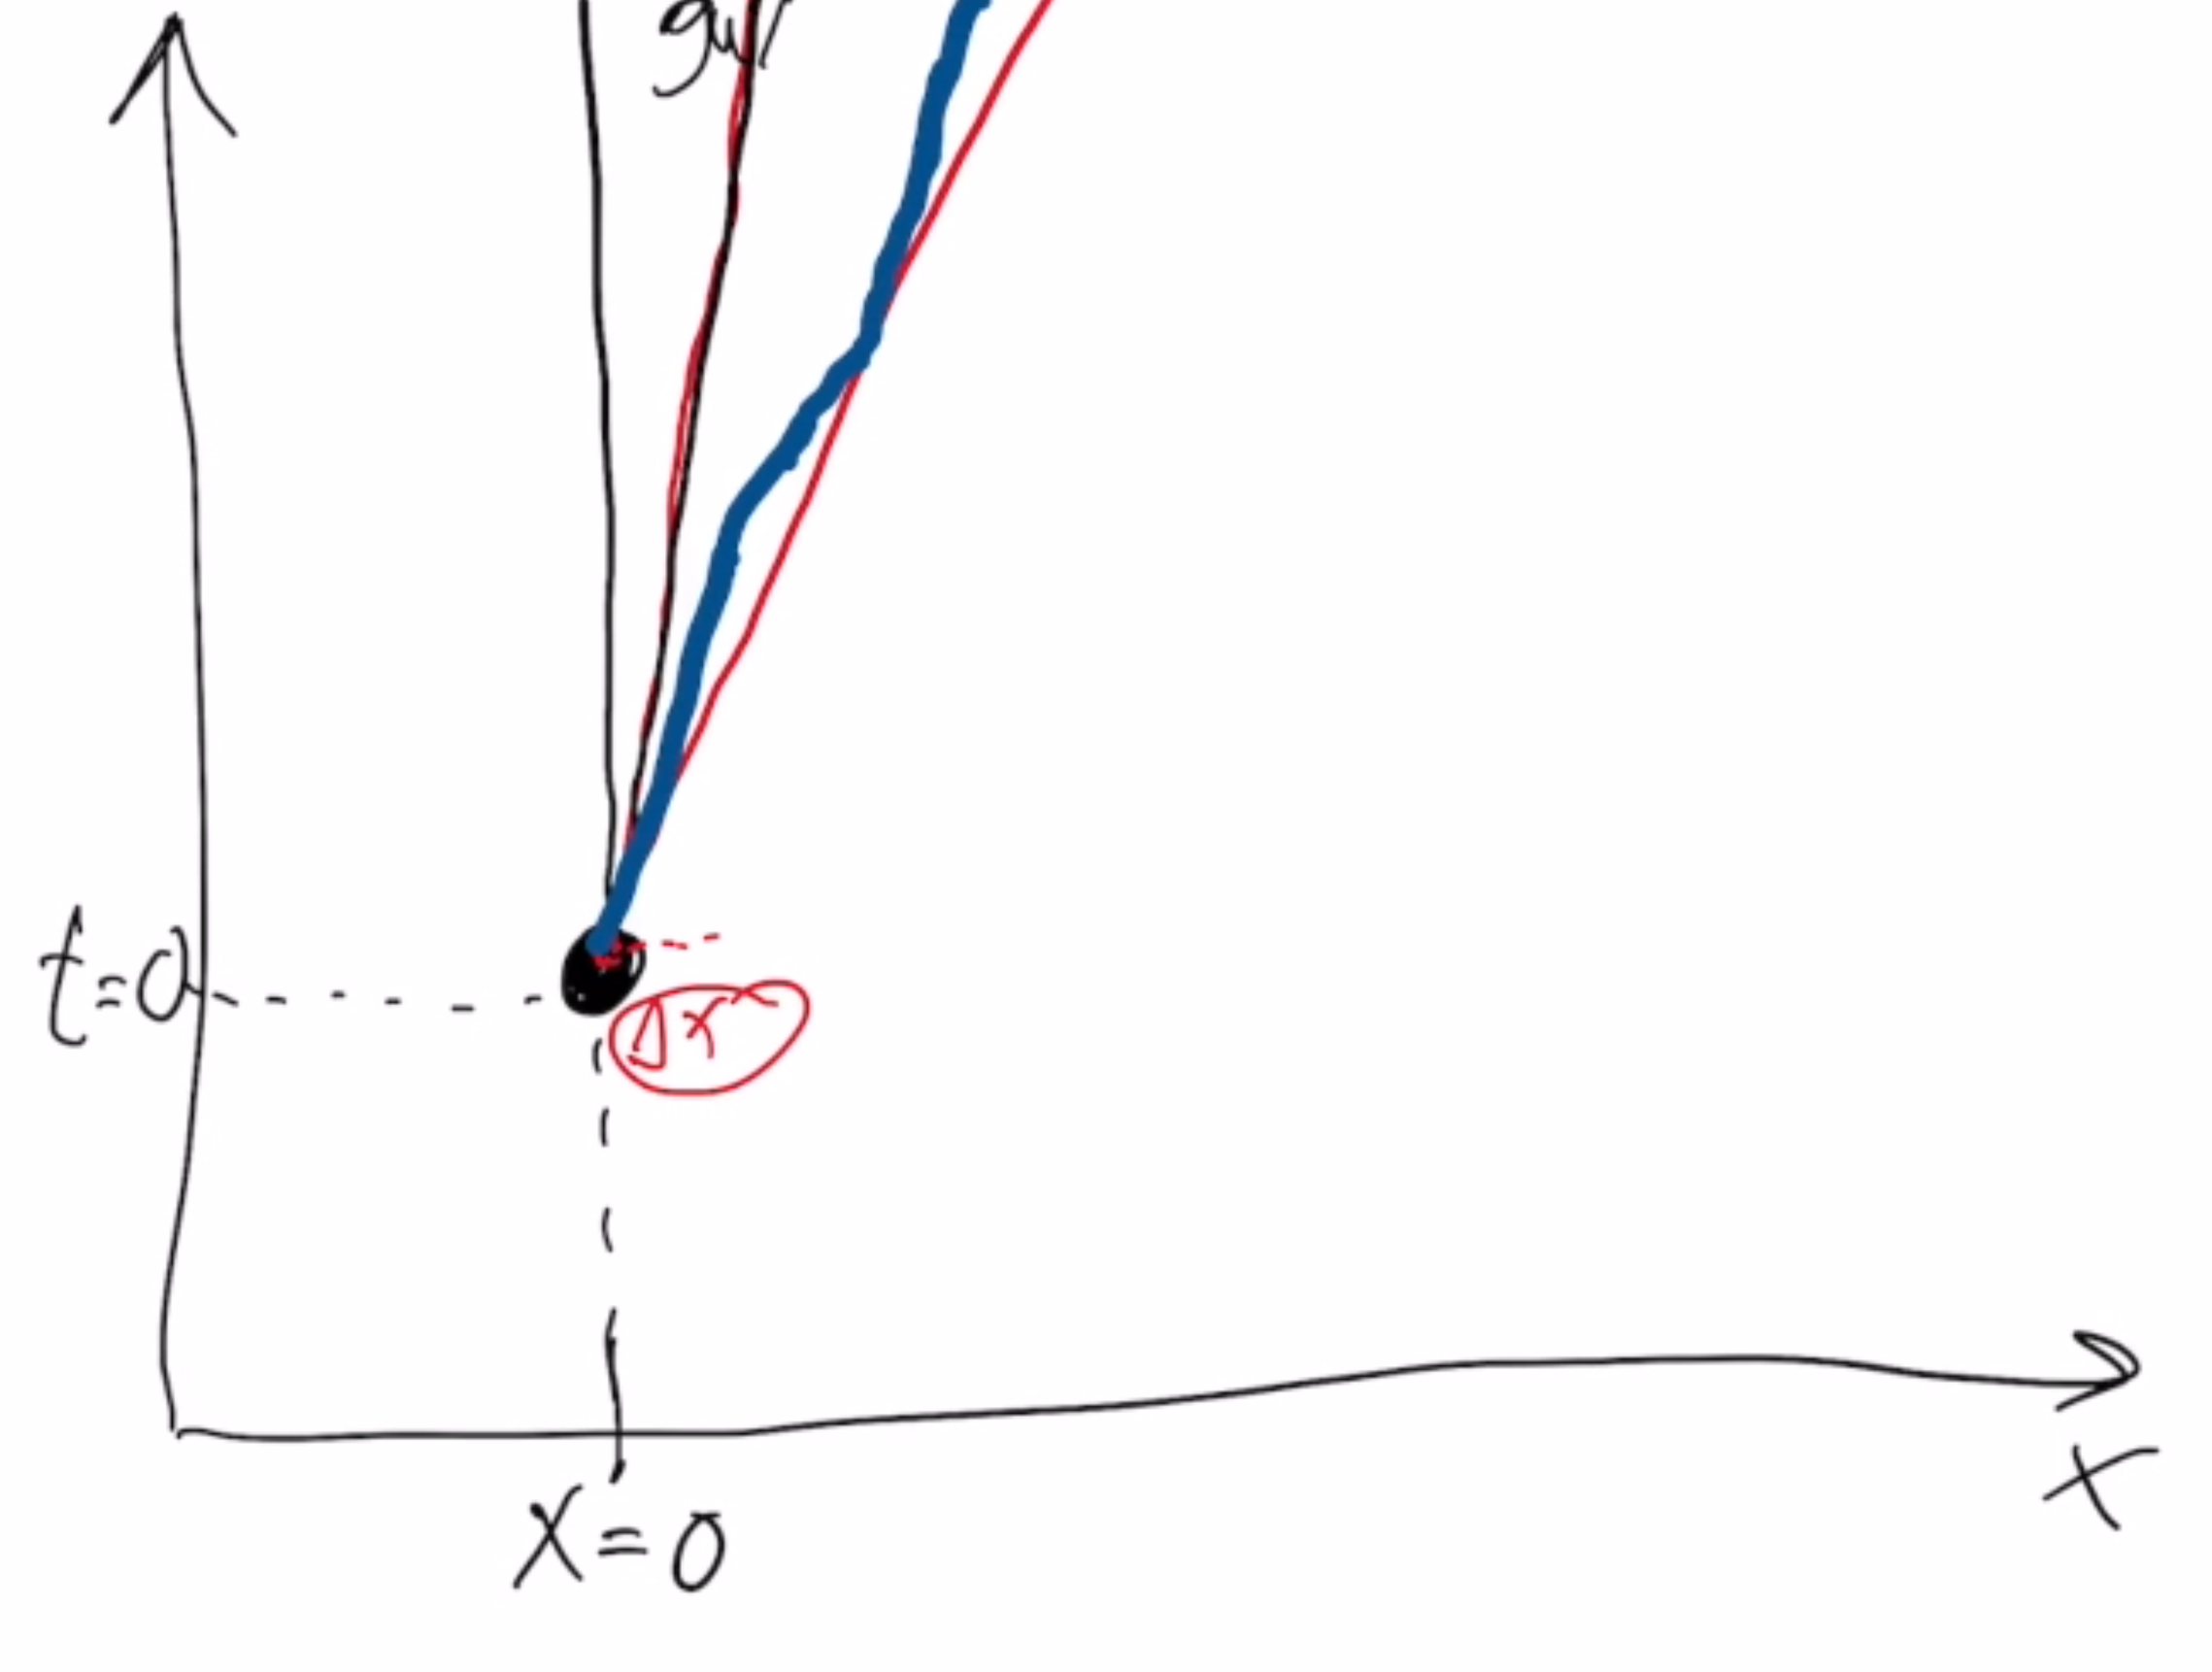
\includegraphics[scale=0.15]{media/romskipene1.png}}
Hvis du på dette tidromdiagrammet måler eller integrerer opp tidromsavstanden $s$ fra starten til slutten av animasjonen (tidroms-lengden av hele den røde linjen) så får du altså ut nettopp tidromsavstanden $s$ som er den samme i alle referansesystemer.
}

\fullframetxt{td19b}{td19}{td19c}{0}{\footnotesize Neste side}{\footnotesize
Det betyr at hvis du nå går til rødt romskip sitt referansesystem og ser på verdenslinja som du der tegnet for rødt romskip sett fra sitt eget referansesystem:\\
\centerline{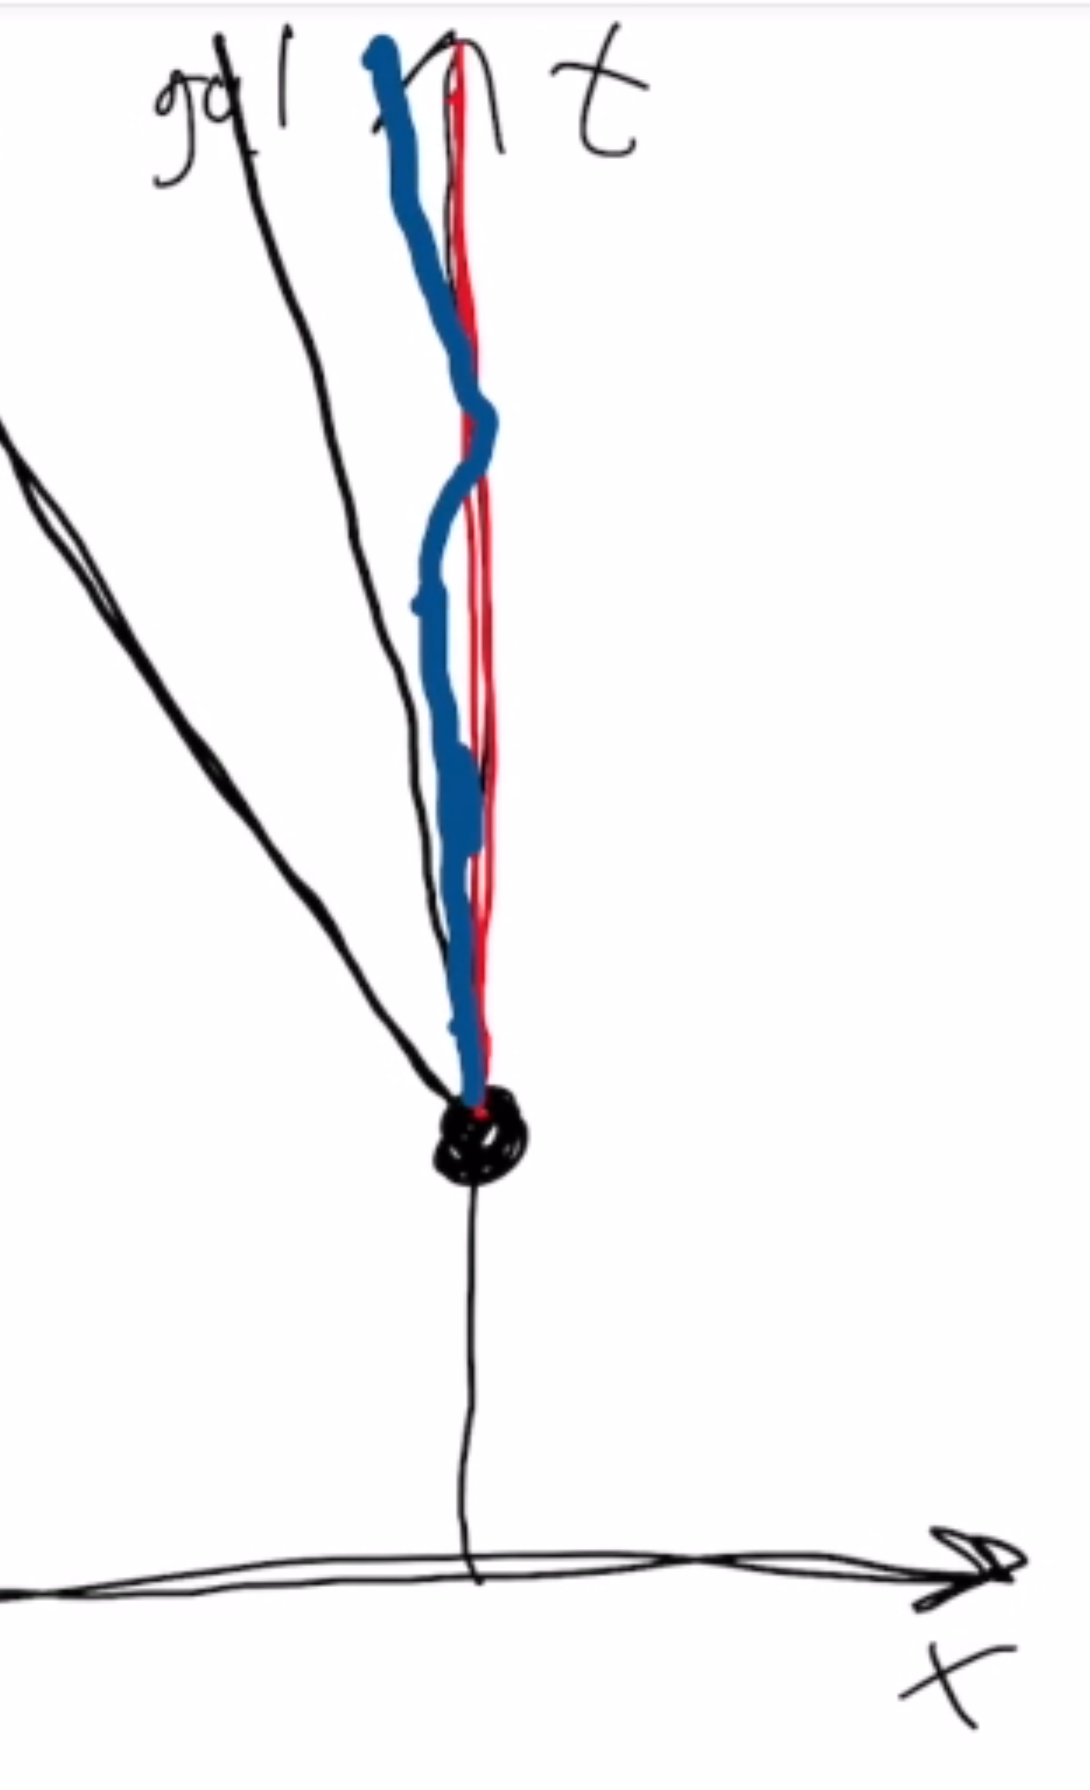
\includegraphics[scale=0.13]{media/romskipene2.png}}
...{\bf så er den like lang.} \textcolor{red}{Tidromsavstanden $s$ for den røde linjen her og i det foregående diagrammet er den samme siden tidromsavstanden er uavhengig av referansesystem.} {\bf Men merk deg noe mer:} i rødt romskip sitt referansesystem så ser vi her at linja bare går rett opp langs tidsaksen. {\bf Det betyr at tidromsavstanden $s$ er et mål på egentida $\tau$. Husk at \textcolor{red}{egentida $\tau$} er et tidsbegrep som er bundet opp til et legeme: Egentiden er tiden målt på klokka i legemets eget referansesystem. Egentiden $\tau$ som har gått mellom to eventer er en tolkning av tidromsavstanden $s$. I eksemplet vårt her så snakker vi da om egentida/tidromsavstanden mellom to eventer som skjer i rødt romskip, et ved starten av animasjonen og et ved slutten.}
}

\fullframe{td19c}{td19b}{td20}{0}{
På eksemplet vårt med toget i del 2A så var egentiden til toget den tiden som ble målt med klokka i toget. Og denne tilsvarer altså tidromsavstanden som toget tilbakelegger, altså lengden av verdenslinja i et hvilket som helst referansesystem. Egentiden kalles ofte for {\bf armbåndsurtid} siden det er tiden som måles når man setter et armbåndsur fast på objektet eller personen man skal måle egentiden til.\\
\textcolor{red}{Det som står her er det svært viktig at du får grepet på! Les en gang til gjennom de 3 siste sidene. Hvis du ikke forstår helt, ta kontakt med foreleser (eller padlet).}
}


\fullframe{td20}{td19c}{td21}{0}{
Vi skal nå se på et svært viktig fysisk prinsipp, {\bf prinsippet om maksimal aldring.} I generell relativitetsteori, del 2C, 2D og 2E, kommer dette prinsippet til å bli svært viktig. Følg derfor nøye med og spør {\bf nå} hvis du ikke forstår! Vi begynner med en problemstilling:
\begin{block}{Event A er at...}
... vi slipper et legeme som har hastighet $v$ og lar det bevege seg fritt uten påvirkning fra noen krefter. Legemet er i {\bf fri flyt} som vi snakket om i del 2A. Hva skjer så videre med dette legemet? La oss si at legemet en tid $\Delta t$ etterpå eksploderer i et event B i en posisjon $\Delta x$ lenger bort langs x-aksen. Hvilken vei i tidrommet har dette legemet tatt fra eventa A til event B? Og hvordan vet vi det?
\end{block}
Altså, hvordan blir verdenslinja til dette legemet fra event A til event B? Og hvorfor slik? Tenk før du blar om!
}


\fullframe{td21}{td20}{td22}{0}{\Huge
  Blir det en rett linje fra A til B i tidrommet? Hvordan visste du det?
}


\fullframe{td22}{td21}{td23}{0}{\Huge
  Rett linje betyr konstant hastighet, ikke sant? Hvorfor konstant hastighet?
}

\fullframe{td23}{td22}{td24}{0}{\Huge
  Var det Newtons første lov du brukte?
}

\fullframetxt{td24}{td23}{td25}{0}{Hæææææææææ?????}{
Einsteins generaliserte (og mye kraftigere) versjon av Newtons første lov, maksimal aldringsprinsippet, lyder
\begin{block}{Prinsippet om maksimal aldring:}
Et legeme i fri fly følger den verdenslinja i tidrommet som gjør at det eldes mest mulig på sin vei. Det vil si at det følger den verdenslinja i tidrommet som gjør at det blir flest mulig tikk på armbåndsuret som står fast på legemet. Altså at {\bf egentida $\tau$} blir størst mulig. Men vi har lært at egentid $\tau$ og tidromsavstand $s$ er en og samme størrelse (dette {\bf må} du ha kontroll på nå!) Det betyr at legemet tar den veien i tidrommet som gjør at tidromsavstanden $s$ blir størst mulig.
\end{block}
}


\fullframe{td25}{td24}{td25b}{0}{\huge
  \textcolor{red}{I \href{https://www.uio.no/studier/emner/matnat/astro/AST2000/h20/undervisningsmateriell/interaktive-forelesningsnotater/2b/videoer/video2b_9.mp4}{denne videoen} diskuterer vi maksimal aldringsprinsippet litt mer og forklarer detaljert hvordan det gir oss Newtons første lov. Se gjerne videoen to ganger slik at du er helt sikker på at du forstår.} {\bf Synes du det er vanskelig å se for seg hvordan den rette linja kan være den lengste mulige? Den første delen av \href{https://www.youtube.com/watch?v=kEB11PQ9Eo8}{denne animasjonen} kan hjele litt på forståelsen.}
}


\fullframe{td25b}{td25}{red_td25c}{0}{
Vi går et øyeblikk tilbake til eksemplet med de 3 bilene som var samlet på et sted i et event A, deretter kjørte med forskjellige hastigheter til de igjen møttes i et event B. Her ser du det igjen i tidrommet:
\centerline{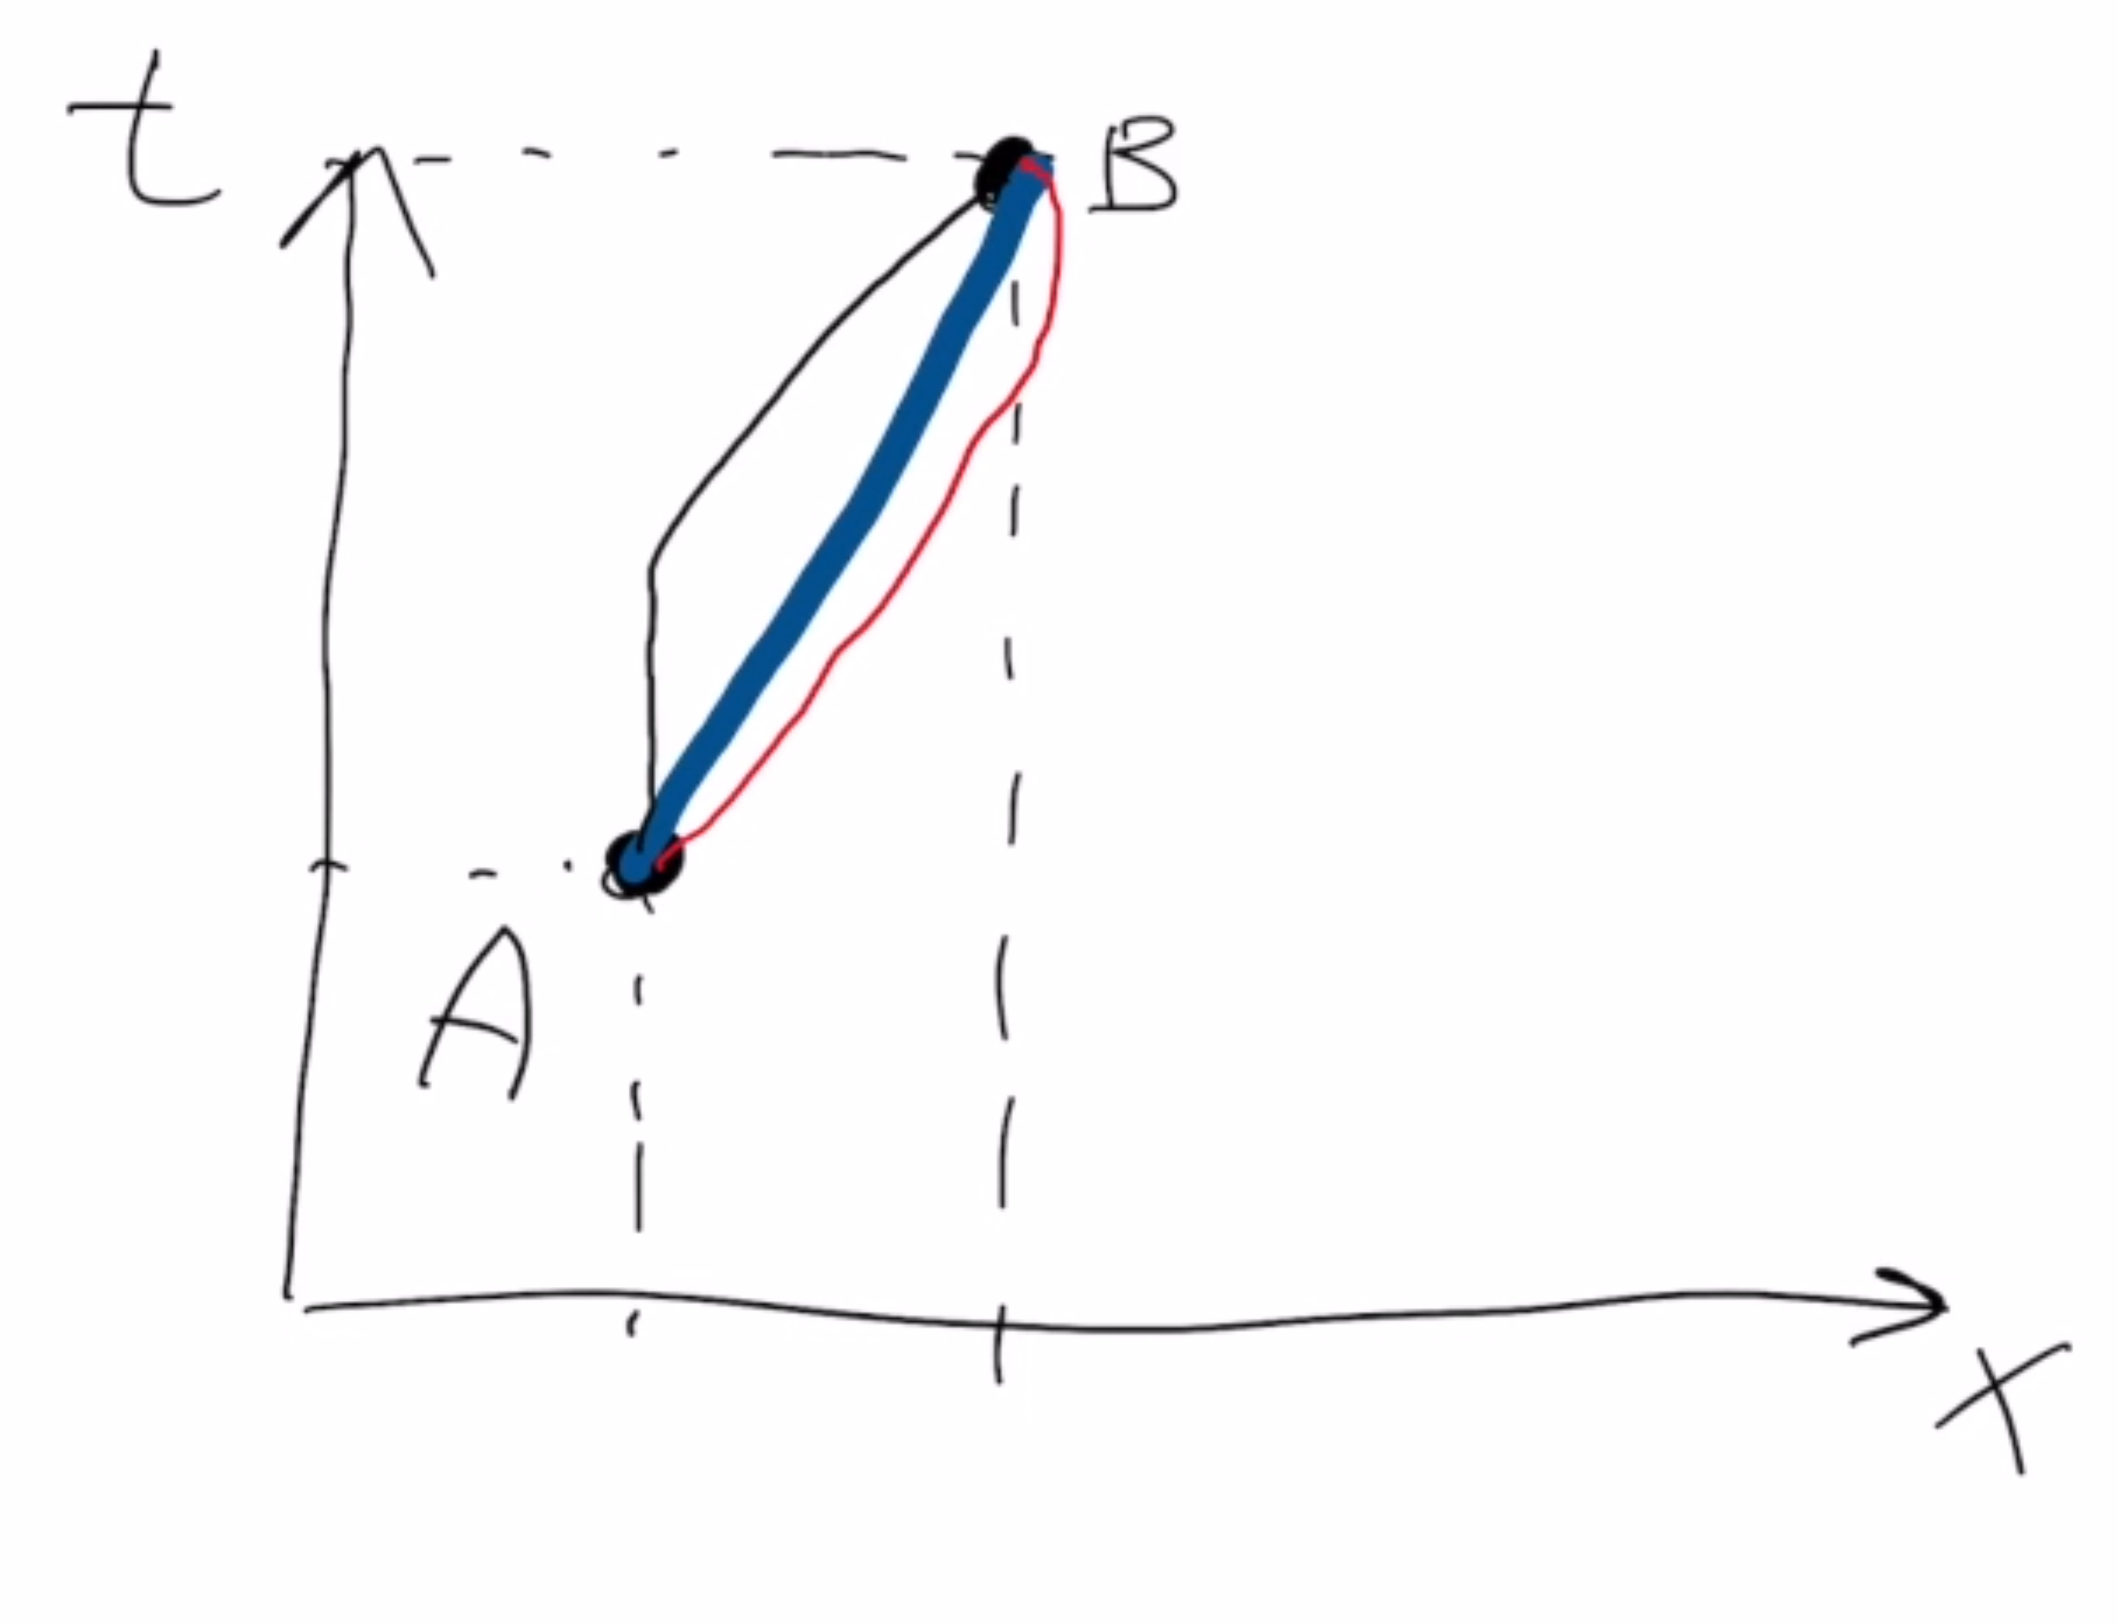
\includegraphics[scale=0.15]{media/cars.png}}
La oss si at det tok 10 sekunder fra A til B i bilen som kjørte med konstant hastighet. Kan du tegne inn en liten prikk på linja med konstant hastighet for hver gang klokka i denne bilen tikker? (regn med at den tikker en gang i sekundet). Tegn deretter også inn tilsvarende prikker på de andre to verdenslinjene. Trenger kun å være kvalitativt rett, altså omtrentlig riktig relativ avstand og antall prikker.
}

\colfullframe{red_td25c}{td25b}{td25d}{0}{red}{\Huge
\textcolor{yellow}{Har du tegnet tidromsdiagrammet med de 3 verdenslinjene og med prikker på? Dette likner på en av ukeoppgavene og flere eksamensoppgaver, så sjansen er stor for at du kommer til å trenge dette. Bedre å lære og forstå det nå!}
}

\fullframe{td25d}{red_td25c}{td26}{0}{\Huge
Når du har gjort et skikkelig forsøk, se på \href{https://www.uio.no/studier/emner/matnat/astro/AST2000/h20/undervisningsmateriell/interaktive-forelesningsnotater/2b/videoer/video2b_10.mp4}{denne videoen}\\
Hvis du vil se et konkret eksempel og litt mer detaljert tolkning av disse strekene på verdenslinja som representerer tikk på egentidsklokka, se på \href{https://www.uio.no/studier/emner/matnat/astro/AST2000/h20/undervisningsmateriell/interaktive-forelesningsnotater/2b/videoer/video2b_10b.mp4}{denne videoen}.
}

\fullframe{td26}{td25d}{pause2}{0}{\large
For å oppsummere:
\begin{itemize}
\item Et legeme i fri flyt som beveger seg en romlig avstand $\Delta x$ i løpet av en tid $\Delta t$ fra et event A til et event B, følger den veien i tidrommet som gir størst mulig egentid, altså flest mulig tikk på armbåndsuret fra event A til event B.
\item Størst mulig egentid betyr størst mulig tidromsavstand $s$ fra event A til event B.
\item I et 4-dimensjonalt tidrom med Lorentzgeometri, er den rette linja den lengste mulige avstanden mellom to punkt. Da følger legemet altså en rett linje i tidrommet.
\item Den rette linja tilsvarer konstant hastighet. Altså må legemet bevege seg fra A til B med konstant hastighet.
\item Dette er samme konklusjon som i Newtons 1.lov. Men i 2C skal vi se hva som skjer når vi ikke lenger har Lorentz-geometri.
\end{itemize}
}

{
\setbeamercolor{background canvas}{bg=cyan}
\begin{frame}
\label{pause2}
\hyperlink{td26}{\pagebutton{\small Forrige side}}
{\huge
\centerline{Kaffe igjen?}
\centerline{
\includegraphics[scale=4]{media/drink-coffee.png}}\\
Dette vasr mye abstrakt tenkning, da trenger vi litt koffein og litt adrenalin: En løpetur ut først, 3 ganger rundt fysikkbygningen så fort du kan! Ikke lov å fortsette før du har løpt alle 3 rundene!
}\\
\vspace*{0.5cm}
\hyperlink{blue_nytema3}{\pagebutton{Ok, jeg er klar for 4D(X?)-matematikk... }}
\end{frame}
}

\renewcommand{\headline}{4-vektorer}
{
\setbeamercolor{background canvas}{bg=blue}
\begin{frame}
\label{blue_nytema3}
\hyperlink{td26}{\pagebutton{\small Forrige side}}
\nytemaside{0}
\hyperlink{vv1}{\pagebutton{La oss begynne med litt 4D-matematikk...}}
\end{frame}
}

\fullframe{vv1}{td26}{vv2}{0}{\label{vektorer}\Huge
Vi begynner med en introduksjon til 4-vektorer i \href{https://www.uio.no/studier/emner/matnat/astro/AST2000/h20/undervisningsmateriell/interaktive-forelesningsnotater/2b/videoer/video2b_11.mp4}{denne videoen}. Se gjerne videoen to ganger til du har full kontroll!
}

\fullframe{vv2}{vv1}{vv3}{0}{\Large
{\bf Anta at vi har en 4-vektor $x_\mu=(t,x,y,z)$ i et umerket referansesystem} og \textcolor{red}{den samme vektoren i et merket referansesystem $x'_\mu=(t',x',y',z')$.} Det kan være en 4-vektor som peker på et event som skjer i posisjon $(t,x,y,z)$ i det umerkede systemet og i posisjon $(t',x',y',z')$ i det merkede systemet. \textcolor{blue}{Det merkede systemet beveger seg med en hastighet $v_\mathrm{rel}$ i forhold til det umerkede.} Transformasjonen beskrives ved \textcolor{red}{Lorentzmatrisen $C_{\mu\nu}$} der $\mu$ og $\nu$ som vanlig er indekser over alle 4 dimensjoner, tid og rom. {\bf Kan du skrive opp Lorentztransformasjonen med $C_{\mu\nu}$ som en likning med summetegn?} Altså en matematisk relasjon mellom $x_\mu$ og $x'_\mu$? Ikke gå videre før du har en sammenheng.
}

\fullframe{vv3}{vv2}{vv4}{0}{\large
Fikk du...
\pagequestion{vv3b}{ja, fikk du...}{-1}
\[
x_\mu'=\sum_{\nu=0}^3C_{\mu\nu}x_\nu
\]
der $\nu$ er summevariabel som summes over 0 (tid) og rom (1, 2, 3)??\\
Einstein ble litt lei av å skrive summer slik at han innførte
\begin{block}{\bf Einsteins summekonvensjon.}
Hvis det i et produkt er to like indekser så skal det egentlig stå et summetegn der, men vi dropper å skrive det. Hvis de to like indeksene er greske, er summen over både tid og rom. Hvis indeksene er latinske er summen over kun romlige indekser.
\end{block}
Da kan likningen vår forenkles til
\[
x_\mu'=C_{\mu\nu}x_\nu
\]
der det altså egentlig er en sum over $\nu$ som vi ikke skriver.
}


\fullframe{vv4}{vv3}{vv5}{1}{\large
Kan du nå skrive det vanlige vektorskalarproduktet
\[
\vec{x}\cdot\vec{y}=
\]
ved hjelp av Einsteinkonvensjonen?
\pagequestion{vv4b}{ja, det blir...}{-2}
\[
\vec{x}\cdot\vec{y}=x_iy_i
\]
Her skriver vi komponentene til vektorene, $x_i$ og $y_i$ med latinske indekser for å markere at de er vanlige romlige 3D-vektorer. Og siden det er produkt med to like indekser (begge er $i$) så er det egentlig en sum.
}

\fullframe{vv5}{vv4}{vv6}{2}{\large
Når vi først er igang med nye konvensjoner, så skal vi se på {\bf det 4-dimensjonale skalarproduktet i tidrommet}. For å markere at man tar et skalarprodukt i tidrommet, skriver man det som en sum med Einsteinkonvensjonen, men en indeks setter man oppe og en nede: $x_\mu y^\mu$ er skalarproduktet i det 4-dimensjonale tidrommet med 4-vektorene $x_\mu$ og $y_\mu$. Merk at det er samme indeks, så det er en sum, men siden det er et 4D-skalarprodukt (en indeks oppe og en nede), skal summen gjøres på følgende måte:
\[
x_\mu y^\mu=x_0y_0-x_iy_i=x_0y_0-\sum_{i=1}^3x_iy_i
\]
der $x_0$ og $y_0$ er tidskomponentene til 4-vektorene mens $x_i$ og $y_i$ er de romlige vektorene. {\bf MERK deg minustegnet mellom tid- og romdelen!} Det er dette som skiller skalarproduktet i 4D-tidrom fra vanlig skalarprodukt!
}

\fullframe{vv6}{vv5}{red_oppsummering0}{0}{
{\bf Det er også minustegnet som er årsaken til at vi skriver en indeks oppe og en nede for å markere skalarprodukt med Einsteins summekonvensjon!}. Anta nå at du har to eventer A og B. 4-vektoren $x_\mu$ peker på event A og 4-vektoren $y_\mu$ peker på event B. Avstandensvektoren $\Delta x_\mu$ (tilsvarende $\Delta\vec{x}$ i vanlig 3D-rom) mellom disse to eventene
\[
\Delta x_\mu=x_\mu-y_\mu
\]
Kan du nå skrive tidromsavstanden $\Delta s^2$ mellom de to eventene uttrykt ved $\Delta x_\mu$?
\pagequestion{vv6b}{ja, det blir...}{-1}
Er du sikker på at du har forsøkt?
\pagequestion{vv6c}{jada, jada, få se da!}{0}
\[
\Delta s^2=\Delta x_\mu\Delta x^\mu
\]
Ser du nå hvorfor skalarproduktet i 4D-tidrom er definert med et minus mellom tid og rom? Hvis du sliter med å forstå, se om \href{https://www.uio.no/studier/emner/matnat/astro/AST2000/h20/undervisningsmateriell/interaktive-forelesningsnotater/2b/videoer/video2b_12.mp4}{denne videoen} kan hjelpe deg.
}

{
\setbeamercolor{background canvas}{bg=red}
\begin{frame}
\label{red_oppsummering0}
\hyperlink{vv6}{\pagebutton{\small Forrige side}}
\textcolor{yellow}{\Large
{\bf Du er ferdig med forelesning 1 av 2 i del 2B.}. I den fysiske forelesningen rekker jeg av og til også gjennom det første temaet i neste forelesning (som omhandler regneregler for 4-vektorer) på den første fysiske forelesningen. Hvis du føler deg frisk og rask og opplagt nå, hopp gjerne over på forelesning 2 for å gå gjennom akkurat det temaet om regneregler nå (ca. 10 sider). Hvis du derimot har fått nok for idag, vent med det til du skal gå gjennom neste forelesning.
}
\hyperlink{oppsummering}{\pagebutton{Til oppsummeringen}}
\end{frame}
}


\begin{frame}
\label{oppsummering}
\hyperlink{vv6}{\pagebutton{\small Forrige side}}\href{https://nettskjema.no/a/171403}{\Changey[1][yellow]{2} \Changey[1][yellow]{-2}}
{\bf Du er ferdig med forelesning 1 av 2 i del 2B.}. Du bør nå:
\begin{itemize}
\item vite hva en verdenslinje er og forstå hva verdenslinjas helning betyr
\item kunne tolke bevegelsen til et legeme fra å se på verdenslinja
\item vite forsjellen mellom tidlike, lyslike og romlike eventer og kunne kjenne igjen slike eventer i et tidromdiagram
\item vite hvordan man kan utlede et integral for å beregne veilengden av en verdenslinje i tidrommet og vite hva slags verdenslinje som er den lengste mulige mellom to eventer
\item kjenne prinsippet om maksimal aldring og hva det betyr
\item kunne utlede Newtons 1.lov fra prinsippet om maksimal aldring
\item vite hva en 4-vektor er og hvordan disse transformerer mellom referansesystemer
\item kjenne Einsteins summekonvensjon og skalarprodukt for 4-vektorer
\end{itemize}
\textcolor{red}{Flott hvis du nå kan klikke på smilefjesene over og fortelle hva du synes om dette interaktive forelesningsnotatet. Hva var bra og nøyaktig hva kan forbedres? All ris og ros mottaes med takk!}
\end{frame}



\end{document}
